\documentclass[aps,prb,a4paper,twocolumn,noshowpacs,superscriptaddress,floatfix]{revtex4}

\usepackage{graphicx}

\usepackage{amsmath}

\usepackage{amssymb}
\begin{document}

\title {Final Report For Logistics Distribution System Location-Routing Modeling}

\author{ϯ�� 516030910487}

\author{����� 516030910483}

\maketitle

\subsection{Motivation}
\subsubsection{Background}
With the development of market economy and logistics technology, physical distribution business developed rapidly.
\subsubsection{Problem}
Consumers need to know the instant logistics information in order to predict the arrival time and pick-up time of express.
\subsubsection{Drawbacks}
Logistics information updates provided by the shopping websites are not timely or the estimated arrival time is inaccurate.
\subsubsection{What to do}
(1)Determine the relationship between logistics distance and approximate time required.
(2) Determine the distribution vehicle scheduling scheme after arriving in the destination city.
(3) Determine the location of distribution points and whether the carrying capacity meets the requirements.
\subsection{Problem formulation}
\subsubsection{The relationship between distance and time}
In physical distribution business, the logistics time from departure to destination is mainly determined by distance and means of conveyance and can be revised by the average timeliness data of the express company in the past few months. The distance and total time spent in the history of express delivery can be counted as a correction parameters.
\subsubsection{Vehicle scheduling problem}
After the express arrives the destination city, the vehicle scheduling problem affects mostly on raising service quality and timelines.
\subsection{Brief introduction of the algorithm}
Our algorithm is about how to model a logistics distribution system including Location and routing to achieve the optimal transportation efficiency and the minimum cost.
\subsection{Analysis}
��Logistics distribution center allocation(based on TSP)+��Vehicle routing selection(based on VRP)
For the above two classical problems, we already have genetic algorithm ant colony algorithm and some other algorithms to solve. But there are some obvious shortcomings in these algorithms. For example, genetic algorithm cannot guarantee the maximum probability convergence to the global optimal solution; ant colony algorithm and particle swarm algorithm are easy to produce local convergence  slow convergence speed.
Therefore, we are trying to design an improved ant colony algorithm with high speed convergence.
\subsection{Mathematical modeling}
\subsubsection{Logistics distribution center allocation}
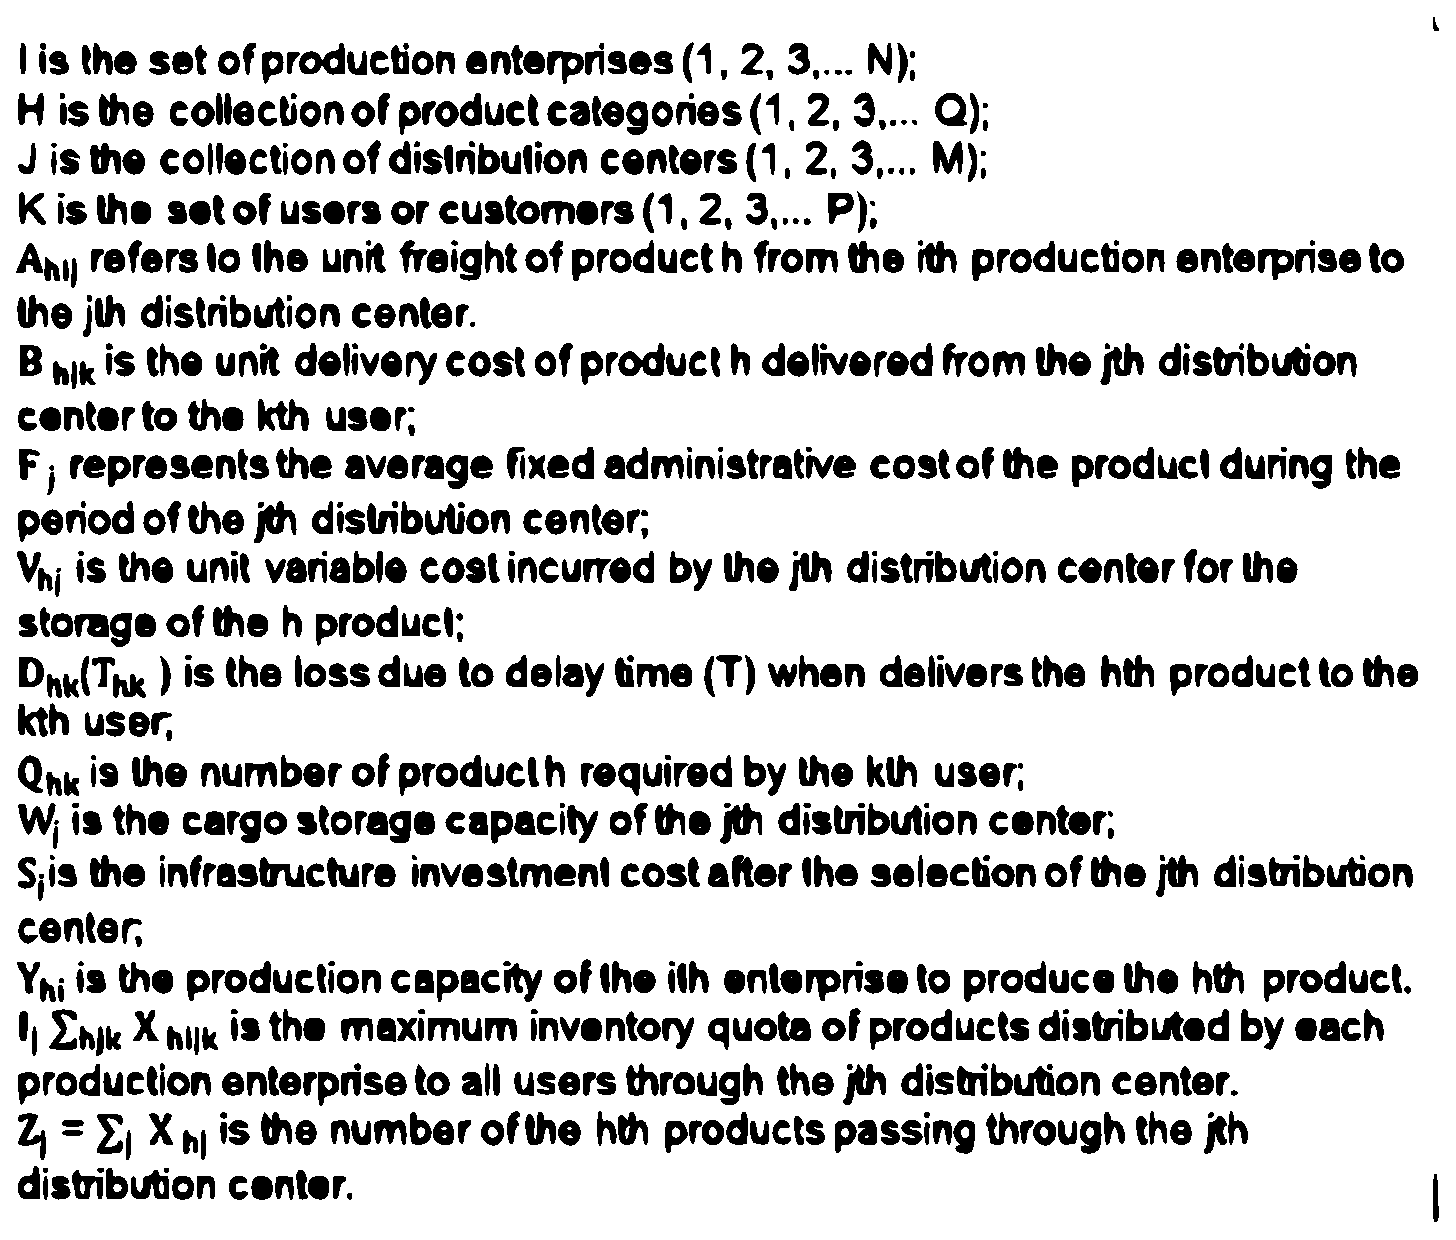
\includegraphics{1}
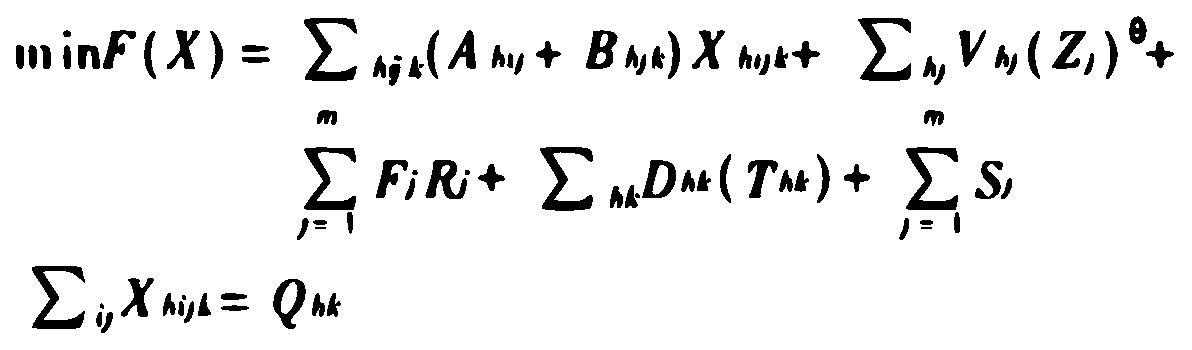
\includegraphics{2}
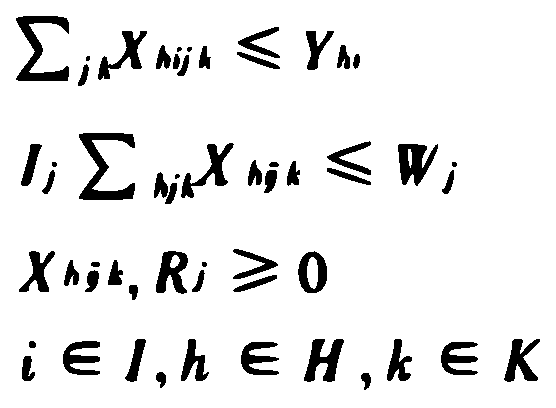
\includegraphics{3}
\subsubsection{Vehicle routing selection}
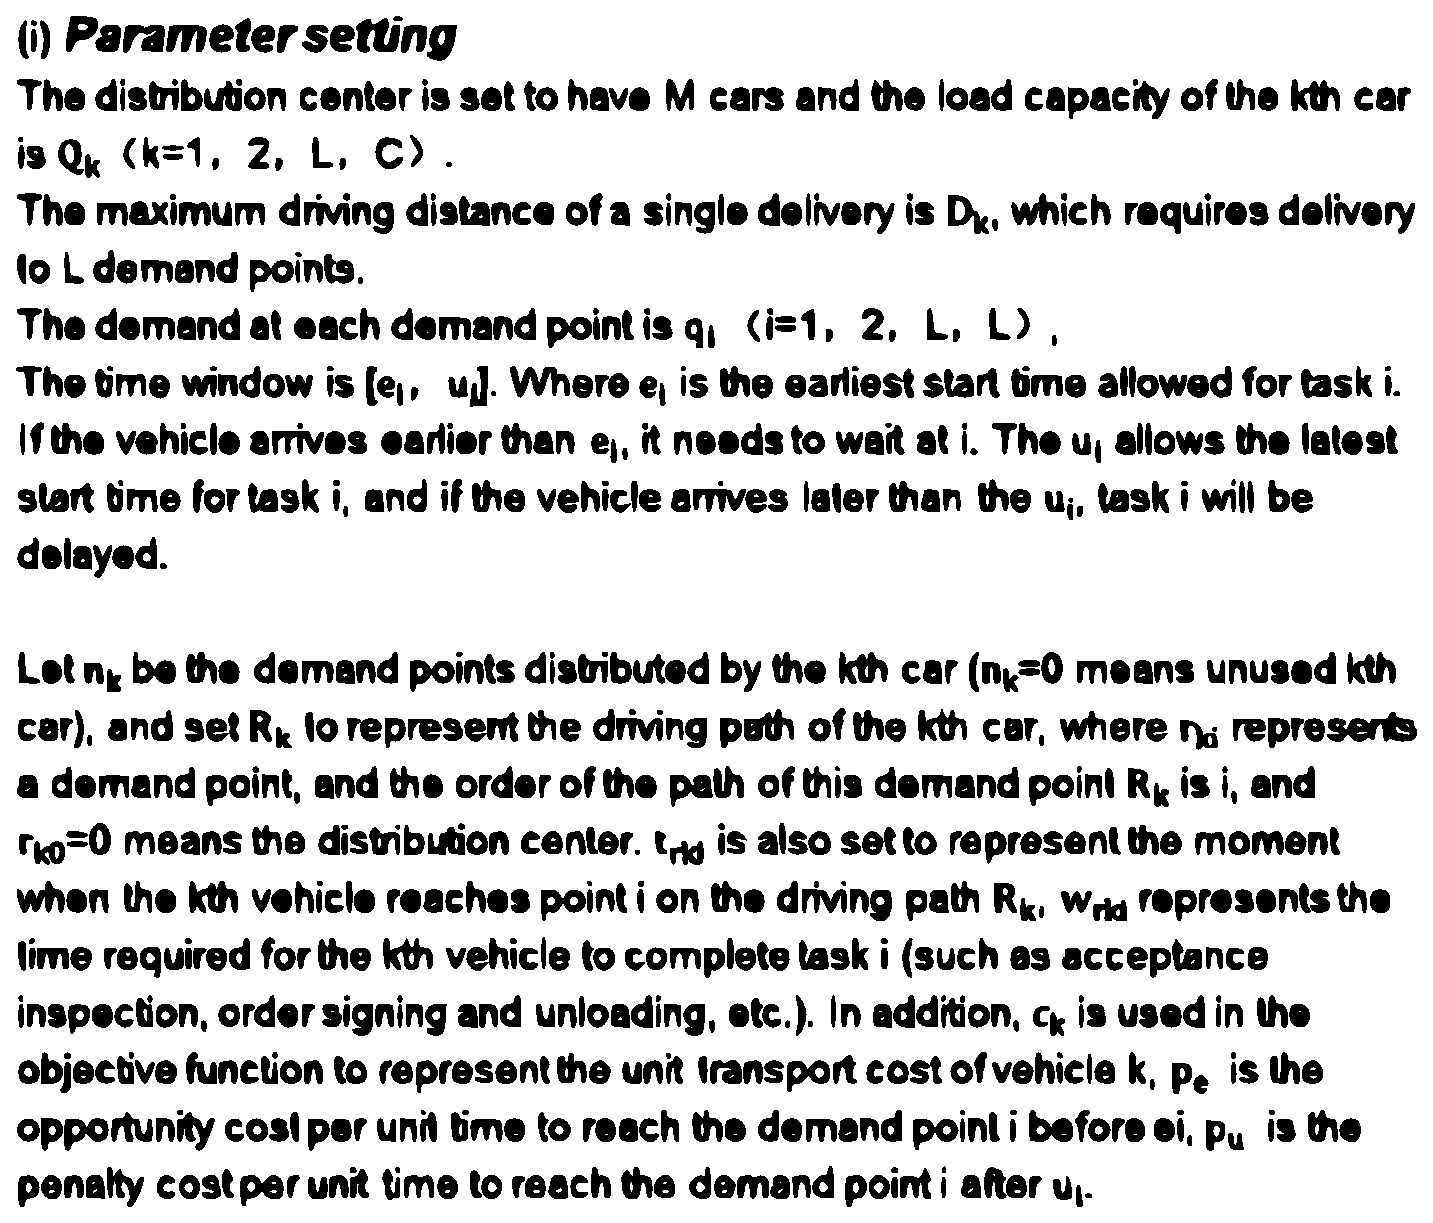
\includegraphics{4}
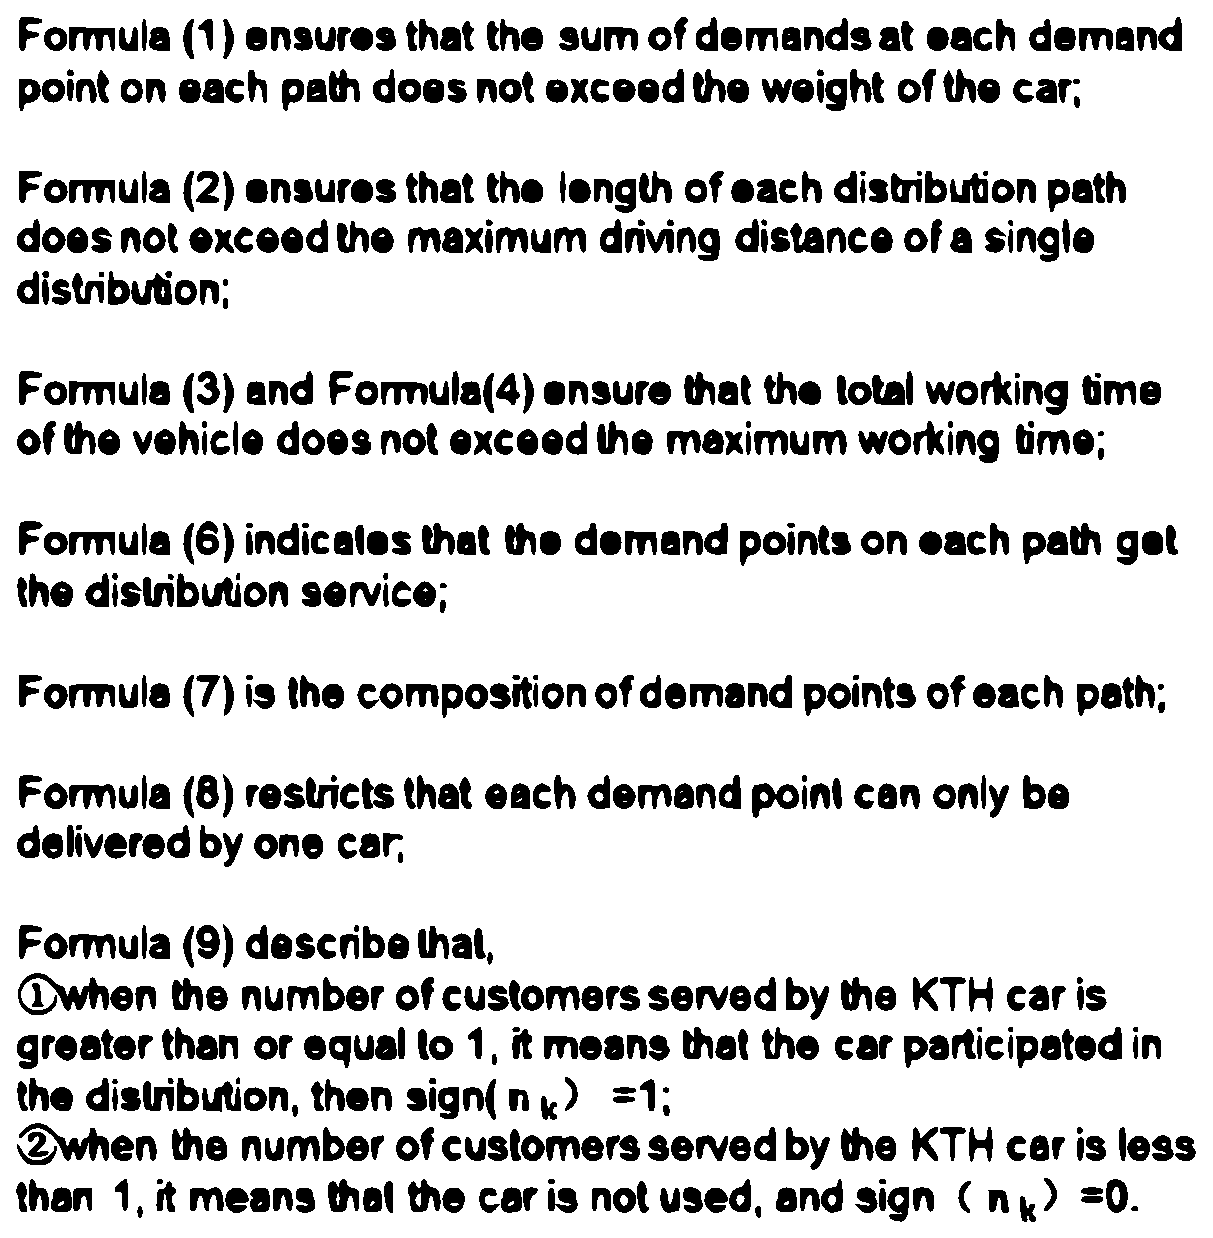
\includegraphics{5}
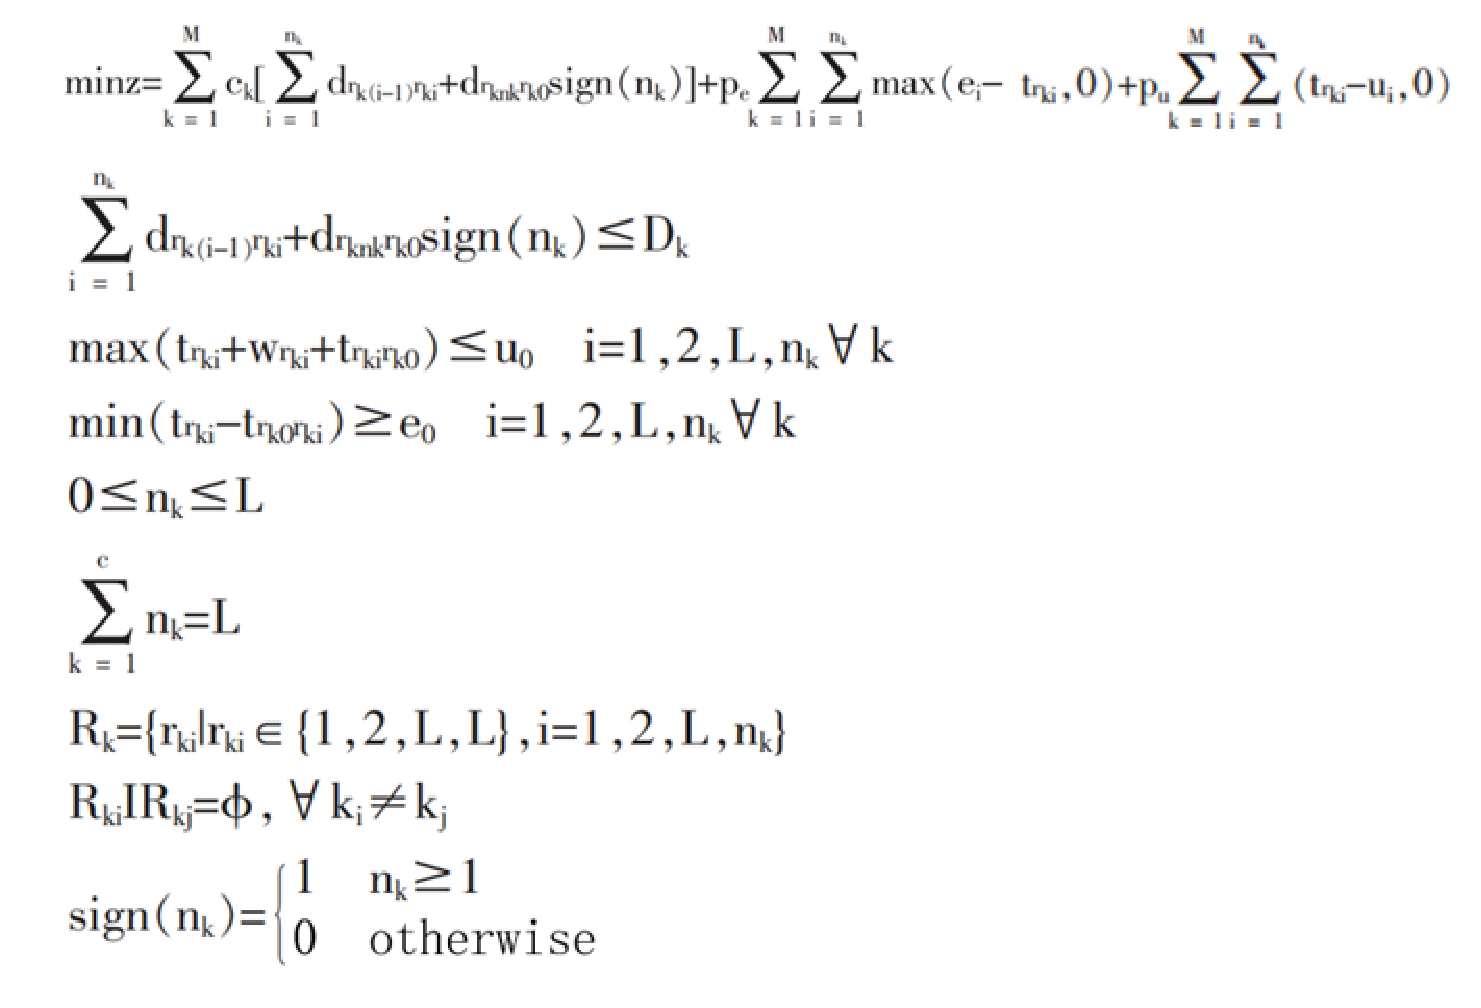
\includegraphics{6}
\subsection{Algorithm design}
Step1: Initialization, setting undetermined parameters and maximum evolutionary algebra;

Step2: Randomly select the location of each ant;

Step3:
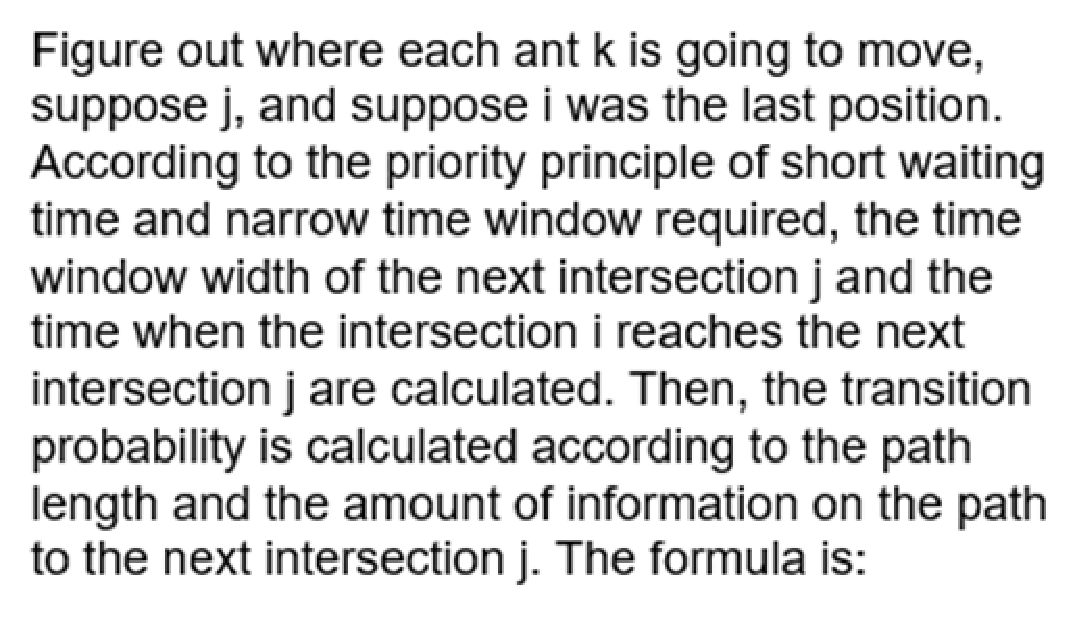
\includegraphics{7}
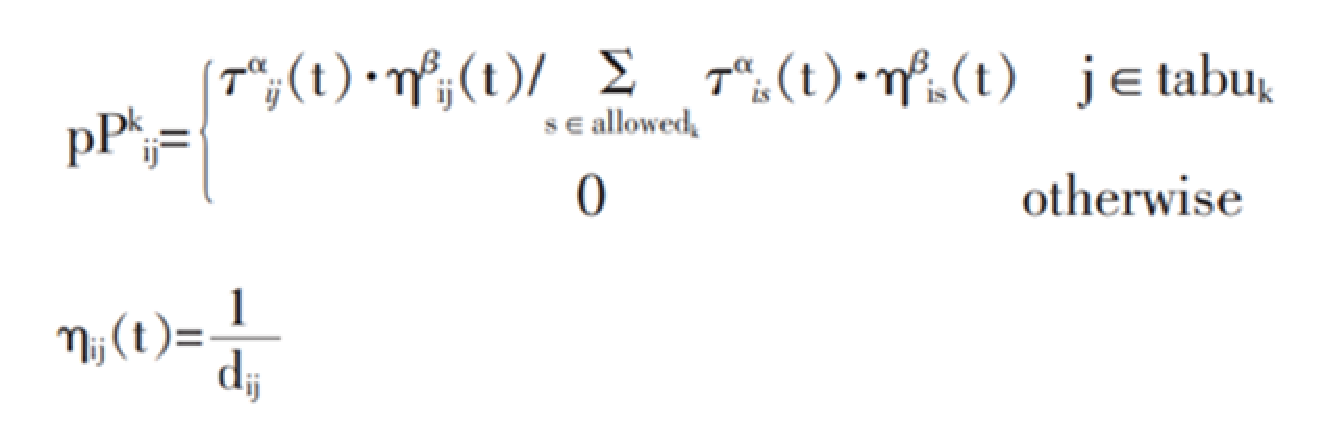
\includegraphics{8}
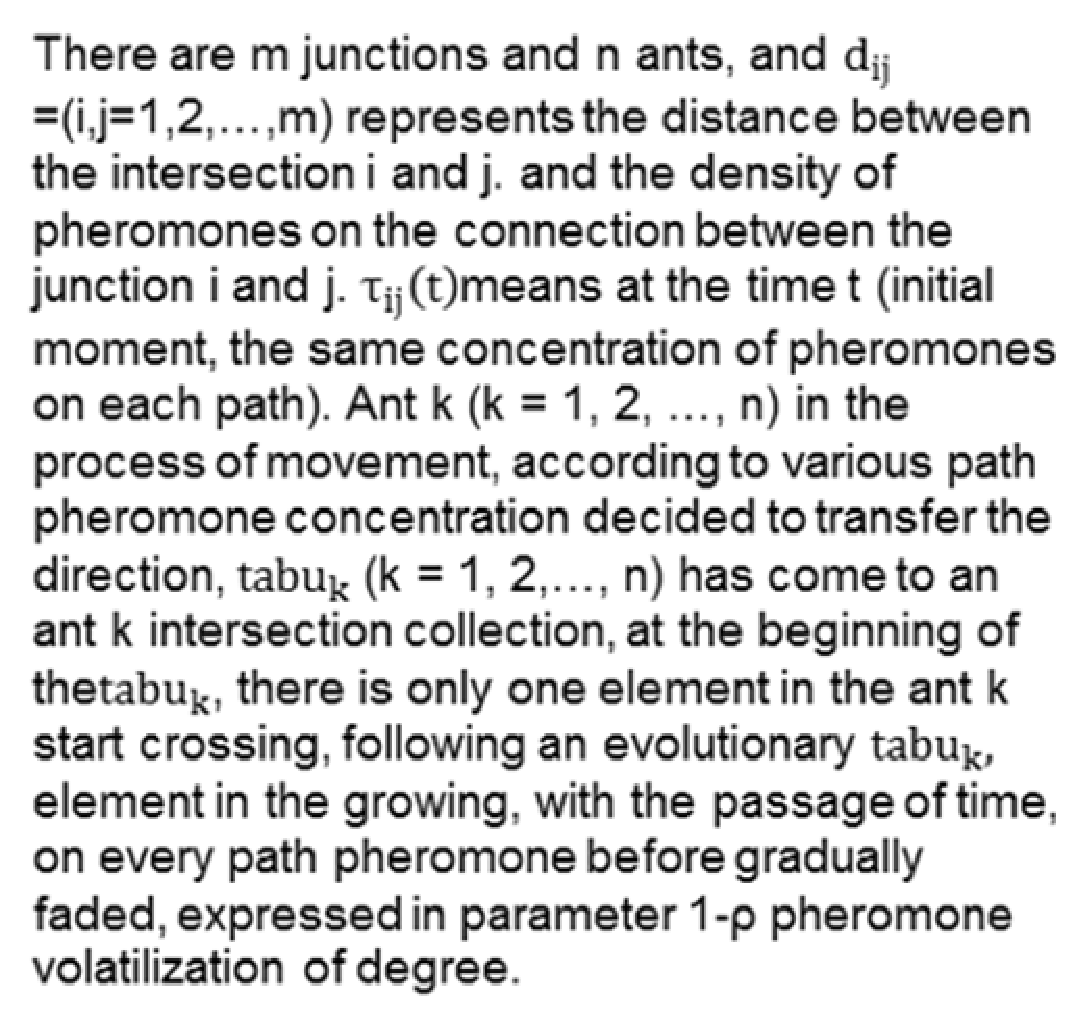
\includegraphics{9}
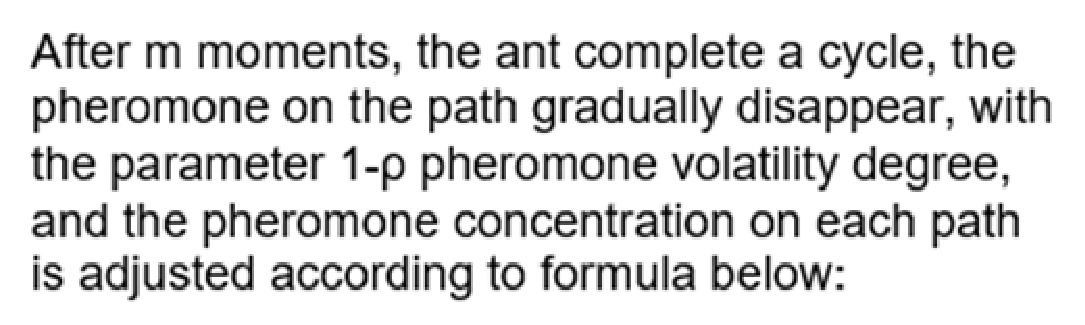
\includegraphics{10}
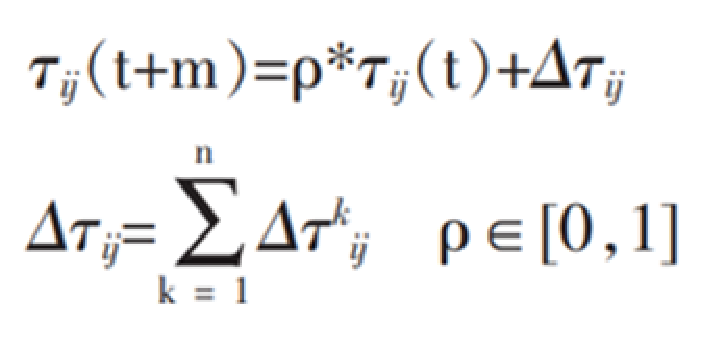
\includegraphics{11}
Step4: Calculate the newly generated pheromone concentration on path ij as follows:
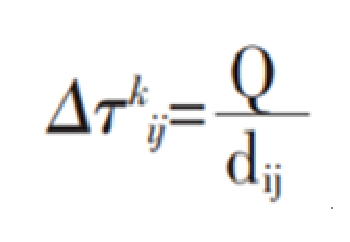
\includegraphics{12}
Q is the pheromone intensity, which is a constant of the number of tracks left by ants, and it affects the convergence degree of the algorithm.

Step5: Calculate the concentration of pheromone diffused from i to il in other paths as follows:
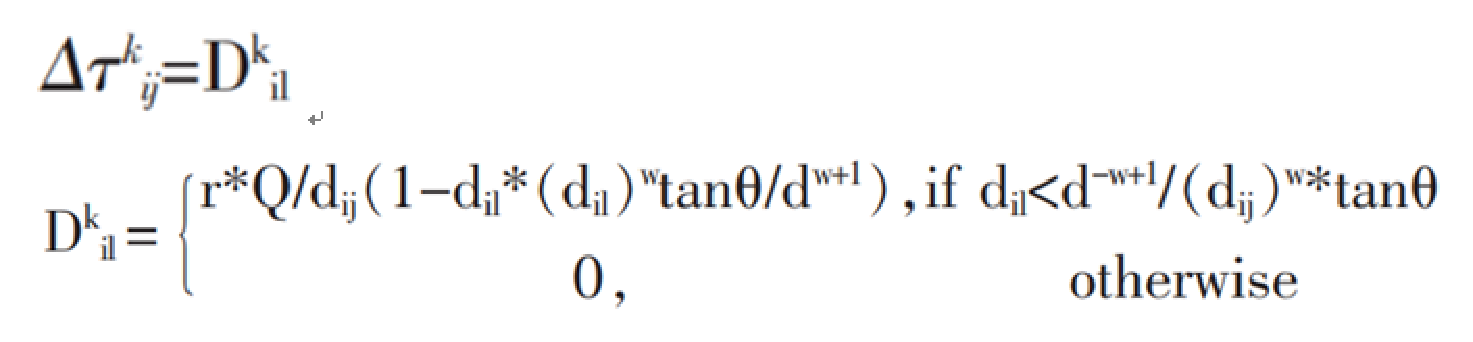
\includegraphics{13}
w is an adjustable constant greater than 1, d is the average distance of cities, r is an adjustable constant less than 1, and the parameter �� is an acute angle.

Step6: Calculate the concentration of pheromone diffused from j to jl in other paths as follows:
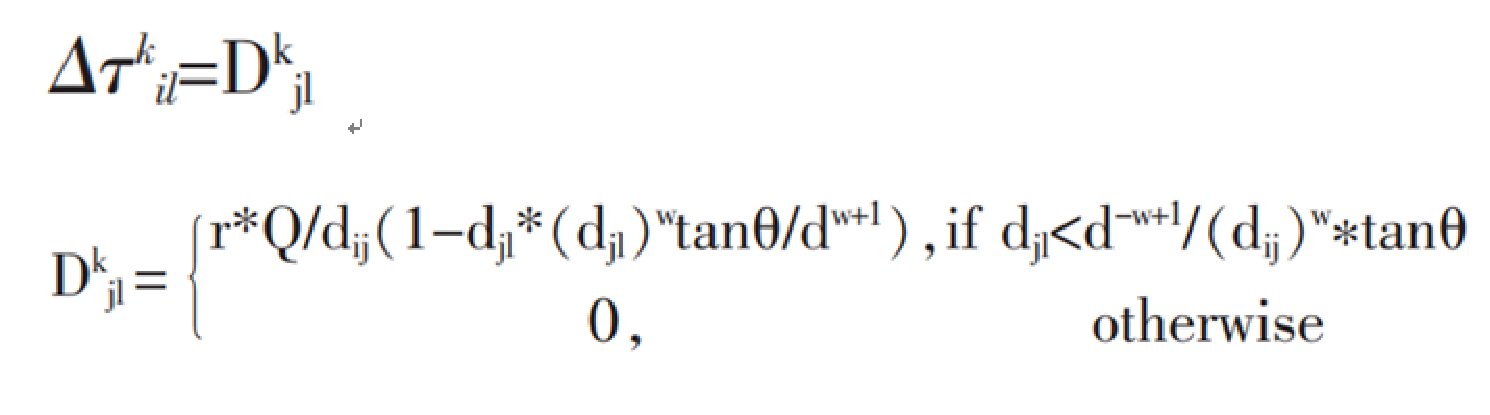
\includegraphics{14}
Step7: If every ant in this cycle has implemented Step3~Step6, go to Step8, otherwise go to Step3.

Step8: Update the pheromone concentration on each path according to equation below�� where m=1.
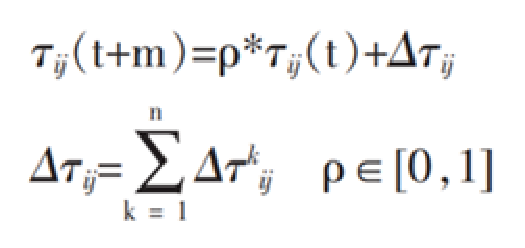
\includegraphics{15}
Step9: If each ant has completed a complete path, turn to Step10, otherwise turn to Step3.

Step10: Judge whether the specified evolutionary algebra has been reached or the obtained solution has not been significantly improved in recent generations, if so, go to Step11, otherwise go to Step3.

Step11: Output the optimization results.
\subsection{Code}
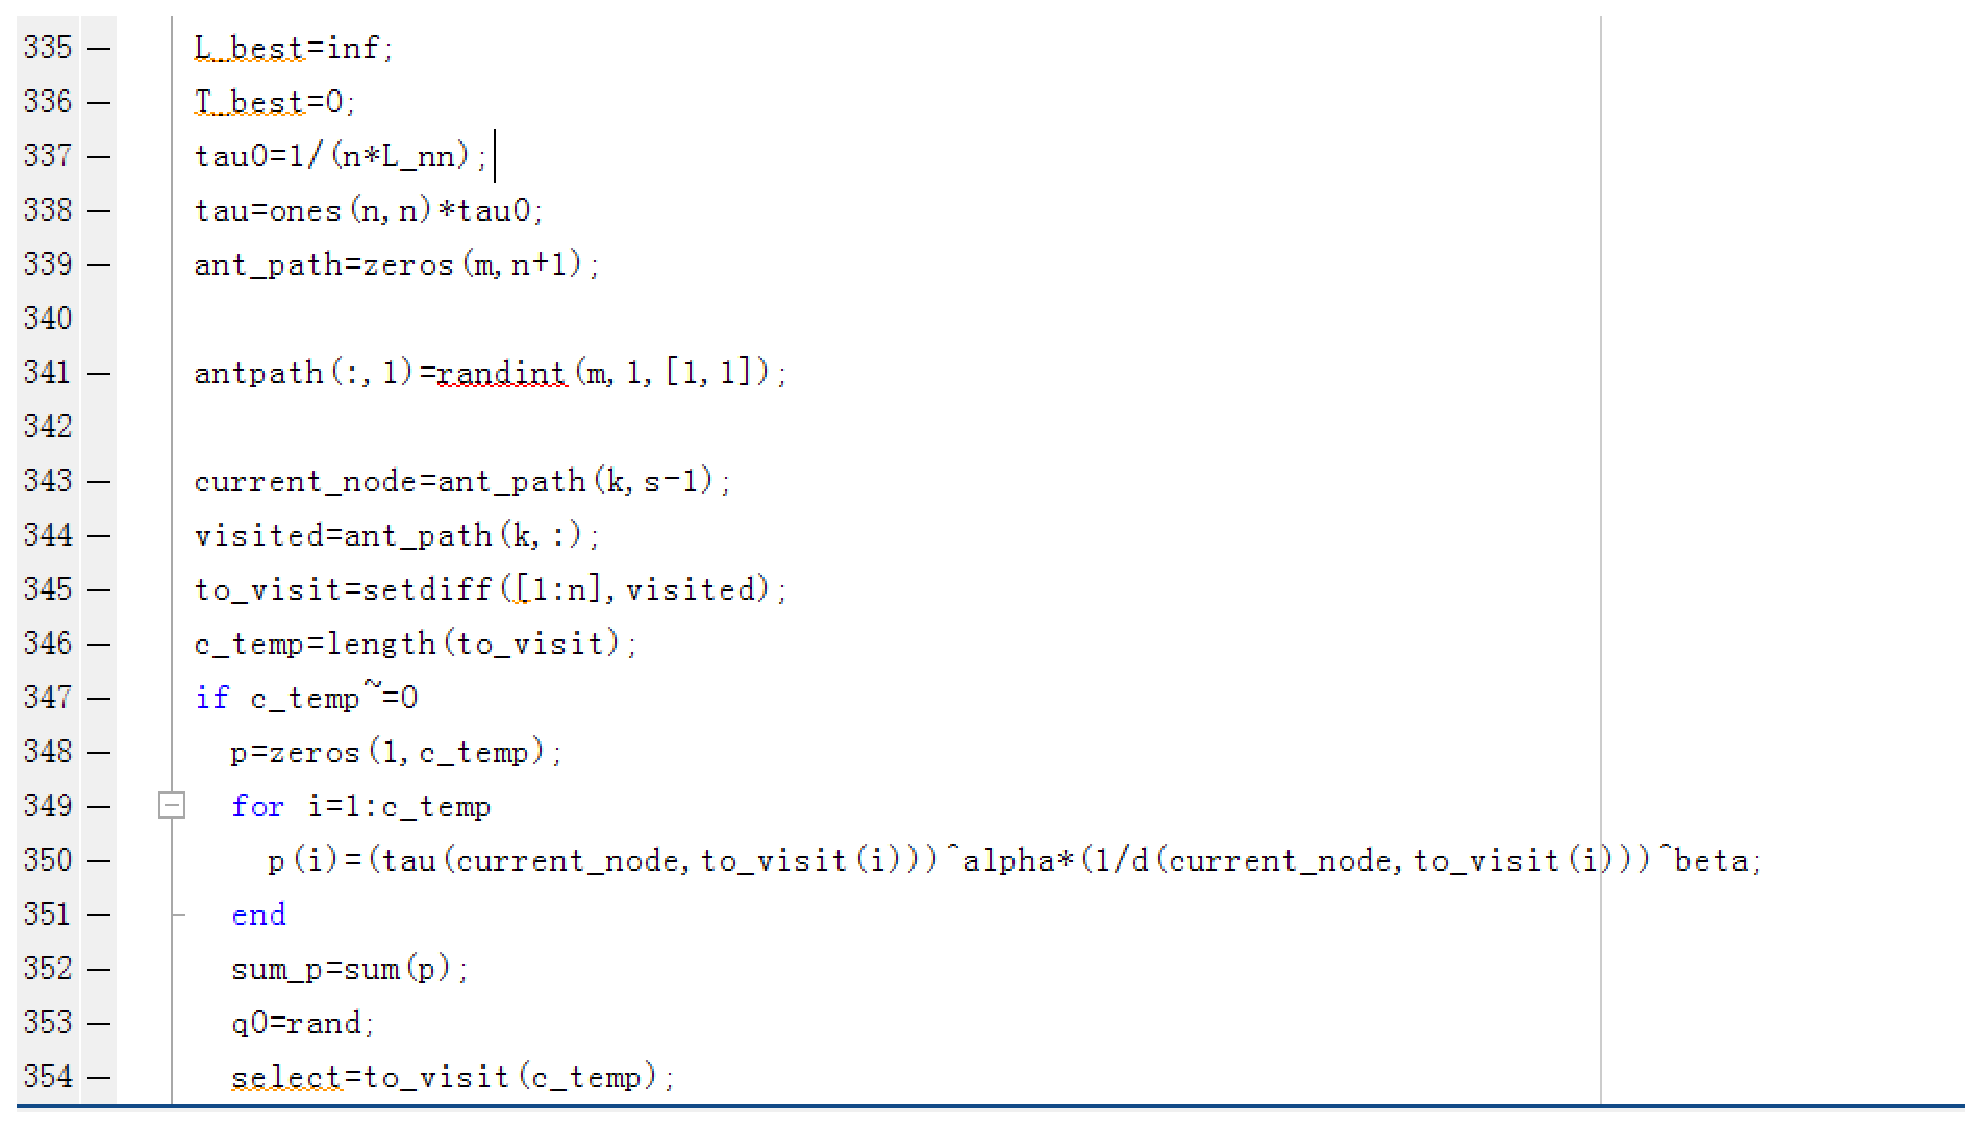
\includegraphics{20}
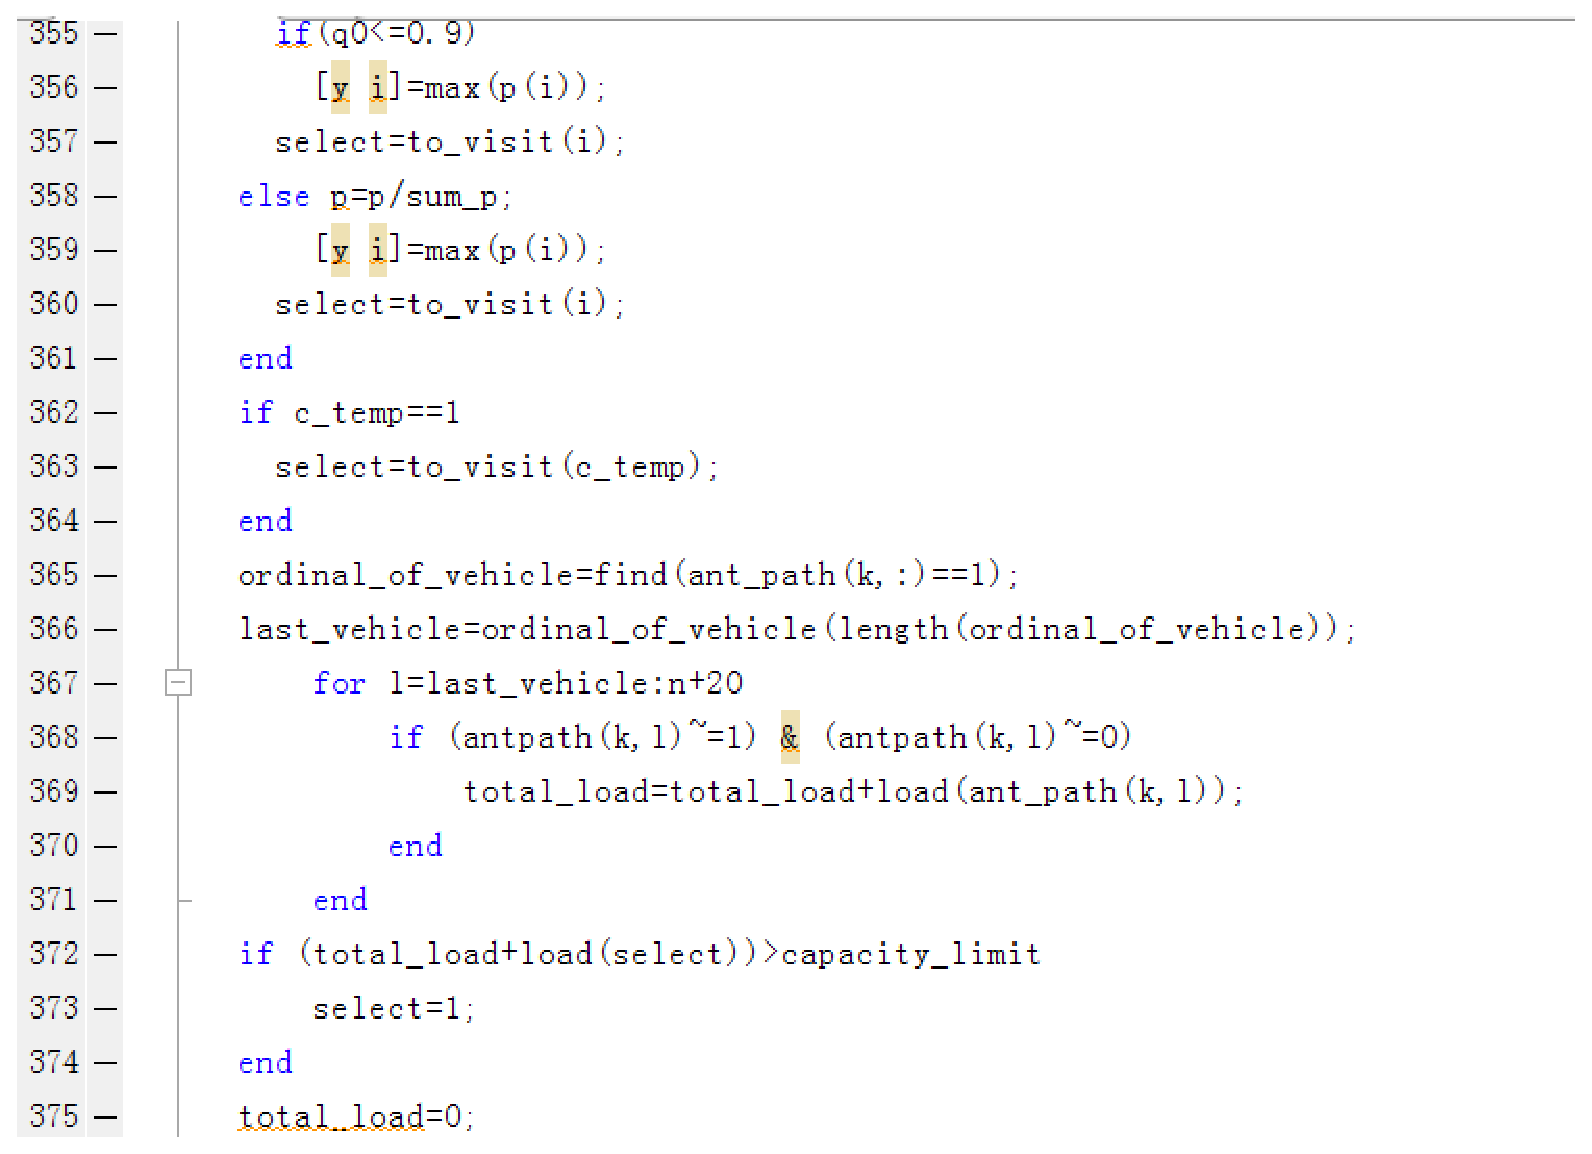
\includegraphics{21}
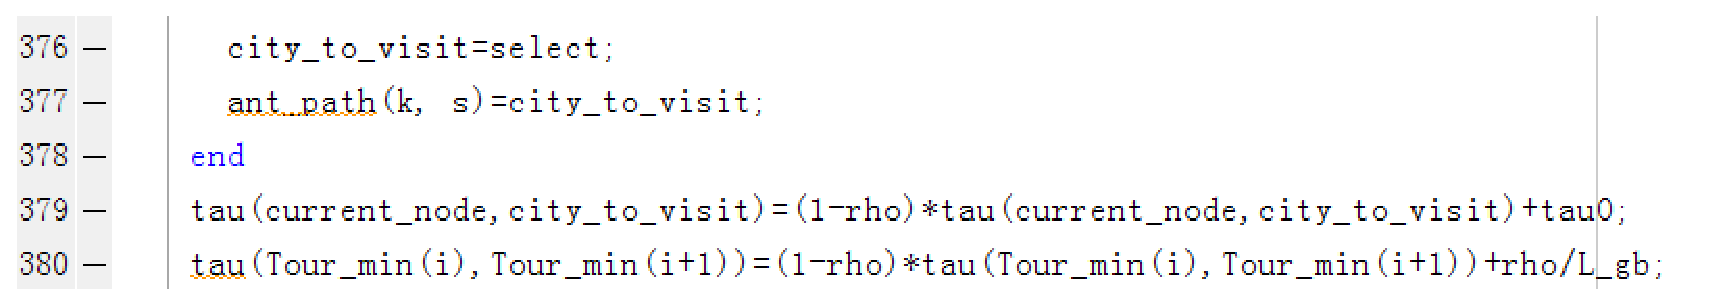
\includegraphics{22}
\subsection{Experiment}
\subsubsection{Consumer location information}
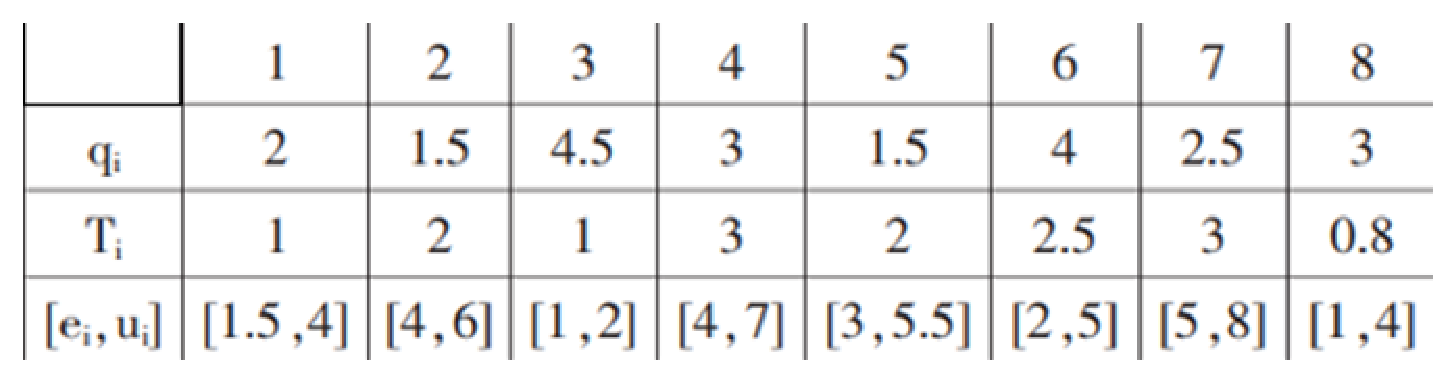
\includegraphics{16}
\subsubsection{Distance between task points and center and between task points}
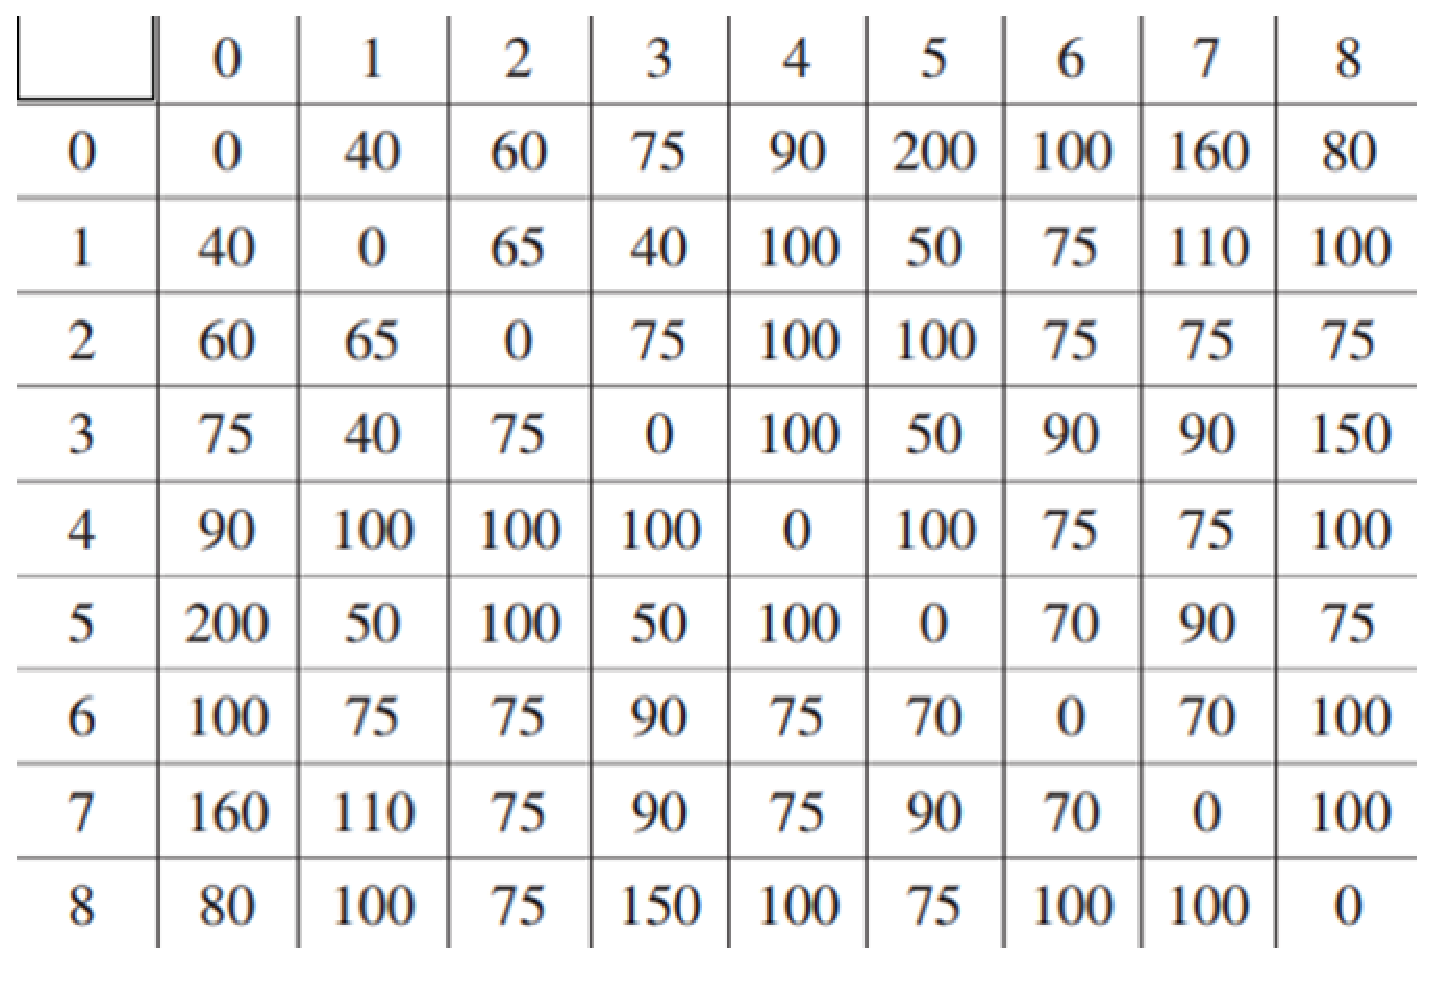
\includegraphics{17}
\subsubsection{Experiment Comparison Results}
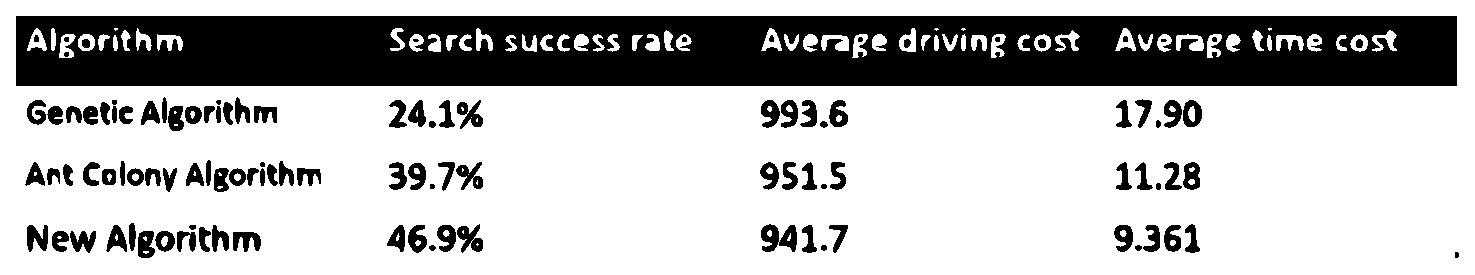
\includegraphics{18}
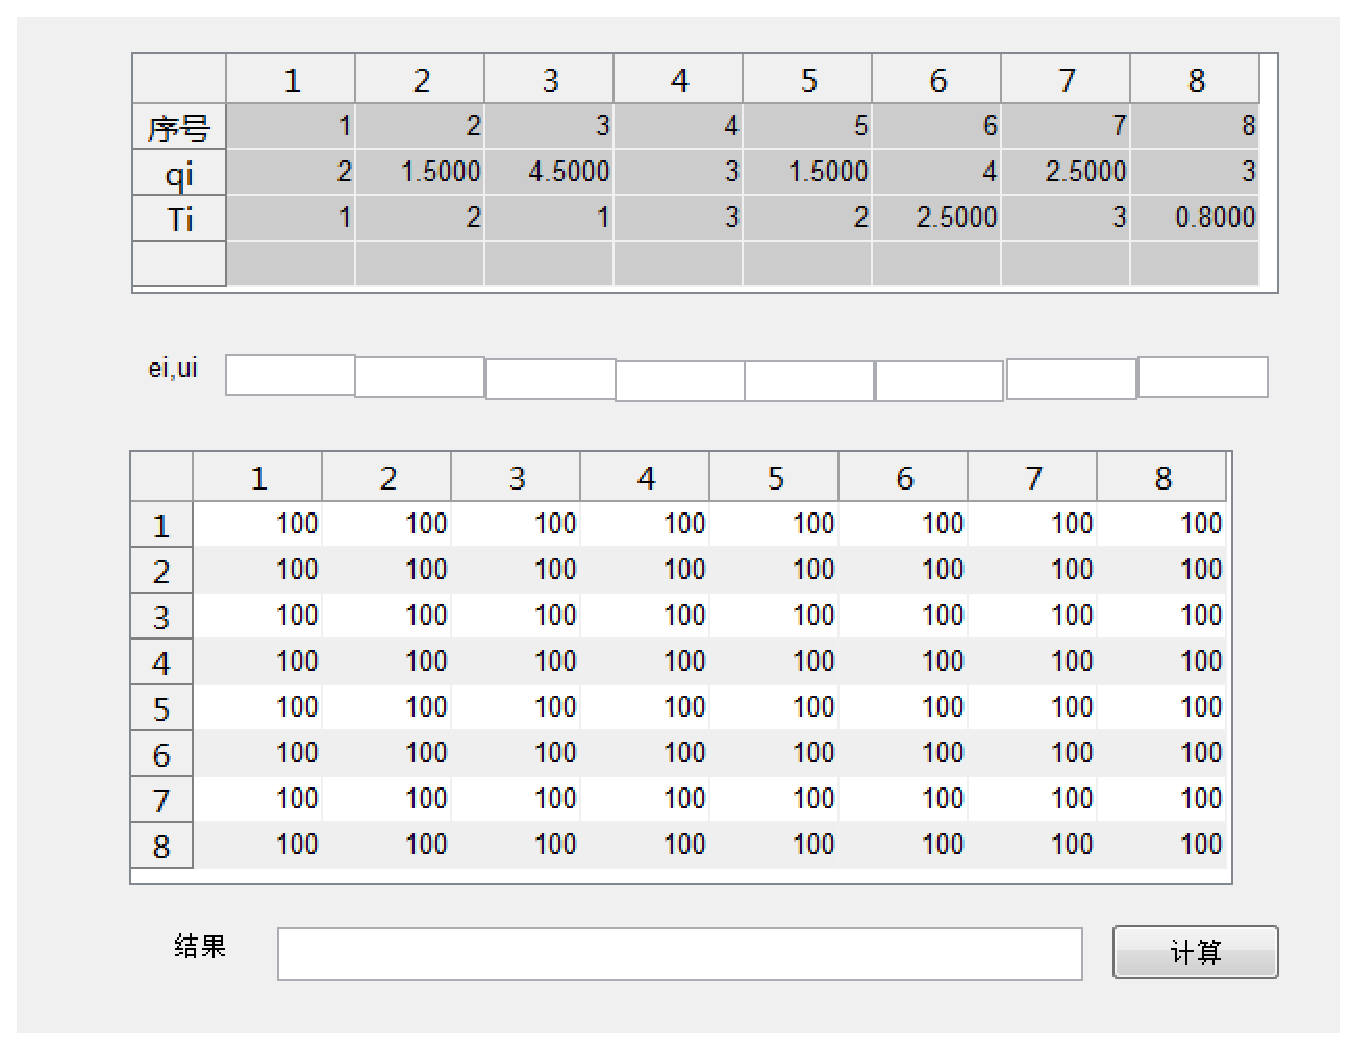
\includegraphics{19}
\subsection{Summary}
An improved ant colony algorithm based on mutation and dynamic pheromone updating is applied to logistics vehicle distribution routing problem with time window constraints. M ants are evenly placed in n edge distribution points, and the nearest neighbor node selection principle is adopted. On this basis, the time window constraints of each intersection are satisfied. At the same time, dynamic local pheromone updating is carried out and mutation algorithm is used to accelerate local optimization and convergence speed. Compared with other algorithms such as genetic algorithm and basic ant colony algorithm, the result of operation on the same computer has obvious advantages. Therefore, the algorithm described in this paper can be used to optimize the vehicle routing of logistics distribution with time window constraints, and the approximate optimal solution can be obtained quickly under the condition of meeting the demand of time windows at each point, which can provide some reference for solving the vehicle routing optimization problem of logistics distribution with time window constraints in the future.    When an ant searches for a path, if it finds a short subpath (subsolution), it releases a corresponding concentration of pheromone. On the one hand, the pheromone directly affects the ants at two points of the subsolution; on the other hand, it will diffuse outward with the path as the center, affecting the behavior of other ants near the path, so that they will have a greater probability in finding the path. Select the path in the next step. At the same time, under the constraints of time windows, ants open new paths to follow the following rules: starting from the last intersection of the current path, to the first intersection of all the unvisited intersections that have the earliest service time. Only when the service time exceeds the time window of the intersection, can we actively open up a new path, and re-restrict the starting point from the untouched intersection, and make the first intersection of all untouched intersections to serve as the first intersection of the latest path. Through this collaborative approach based on pheromone diffusion under time window constraints, on the one hand, it guides ants to open up the next path in meeting the time window of a new intersection, on the other hand, the interference of other ants in choosing the optimal path when choosing the next intersection will be reduced. Thus, the convergence degree of the algorithm is greatly improved while meeting the time window requirements of each intersection, and the search efficiency and success rate of the algorithm are improved.
We programmed the new algorithm with MATLAB, and we found programs using traditional ant colony algorithm. These programs are operated on the same computer. The results of our algorithm are compared with those of genetic algorithm and traditional ant colony algorithm. It is found that the former is obviously better than the latter.
In this algorithm, a new dynamic information strategy is adopted under the premise of meeting the time window constraints of individual points to ensure that each ant contributes to the search in each search. At the same time, a unique mutation strategy is adopted to search each search result in order to search the results of each search. But the logistics distribution center allocation part based on TSP we haven��t found a better algorithm. So in the future we will try to design an appropriate way to solve it.

\end{document}
